\documentclass[a4paper,12pt,twoside]{book}

% Encodage des caractères et langue du document
\usepackage[T1]{fontenc}
\usepackage[utf8]{inputenc}
\usepackage{lmodern}
\usepackage[french]{babel}

\setcounter{tocdepth}{2} % Pour que les subsubsections n'apparaissent pas dans la TOC
\setcounter{secnumdepth}{2} % Pour que les subsubsections ne soient pas numérotées

% Gestions des marges
\usepackage{geometry} 
\geometry{a4paper}
%\geometry{margin=2.5cm}
%\geometry{headheight=6mm}

% Si on a besoin d'une configuration plus précise des marges
\geometry{%
  a4paper,                % format de papier
% Définition des marges :
  left= 3cm,            % marge intérieure à la page
  right = 2cm,          % marge extérieure
  top = 3cm,
  bottom = 3cm,
% En-tête et pied de page :
  headheight=6mm,         % espace réservé à l'en-tête dans la marge top
  %headsep=3mm,            % espace entre le corps et l'en-tête
  %footskip=9mm            % espace entre le corps et le pied de page
}

% Pour une meilleure gestion des maths
\usepackage{amsmath,amssymb,amsfonts,amsthm}
%\usepackage{mathtools} % version modifiée de amsmath, ajoute des symboles, etc.
\usepackage{mathrsfs}% pour rajouter un format de lettres façon "caligraphie" en math mode.

% Pour gérer les unités
\usepackage{siunitx}
\sisetup{inter-unit-product=\ensuremath{{}\cdot{}}} % pour mettre des points médians entre les unités quand il y en a plusieurs
\sisetup{separate-uncertainty=true,multi-part-units=single} % pour faire des incertitudes en écrivant \SI{valeur(incertitude)}{unité}
\DeclareSIUnit\vitesse{\meter\per\second}


% Pour une meilleure gestion des graphiques
\usepackage{graphicx}
\usepackage{caption}
\usepackage{subcaption} % permet de faire des subfigures (remplace le package subfig)

% Pour les tableaux, matrices, listes
\usepackage{booktabs}
\usepackage{array}
\usepackage{paralist} % si besoin regarder "enumitem" qui est un peu différent
%\usepackage{multirow} % pour faire des tableaux plus compliqués

% Pour personnaliser les entêtes et pieds de pages
\usepackage{fancyhdr}
\usepackage{emptypage} % garantit que les pages blanches avant les débuts de chapitres soient vraiment blanches (pas d'entête ni de pied de page)
 
 % On définit le style pour les pages "normales"
\pagestyle{fancy}
\renewcommand{\chaptermark}[1]{\markboth{\chaptername \ \thechapter.\ #1}{}} % sert à personnaliser l'affichage de \leftmark (ici : le mot "Chapitre", le numéro, un point, et le titre du chapitre, sans écrire en majuscules)
\renewcommand{\sectionmark}[1]{\markright{\thesection.\ #1}} % sert à personnaliser l'affichage de \rightmark (ici : le numéro et le titre de la section en cours, sans écrire en majuscules)
\fancyhf{} % assure que les entête et pieds de page sont vides au départ
\fancyhead[LE]{\leftmark}
\fancyhead[RO]{\rightmark}
\fancyfoot[LE,RO]{\thepage}

% On définit le style pour les pages "spéciales" (début de chapitre, table des matières, etc.)
\fancypagestyle{plain}{
\fancyhf{}
\fancyfoot[RO,RE]{\thepage}
\renewcommand{\headrulewidth}{0pt}
\renewcommand{\footrulewidth}{0pt}}

% Explications :
% L = left, R = right, C = center, E = even pages, O = odd pages
%\thepage : adds number of the current page.
%\thechapter : adds number of the current chapter.
%\thesection : adds number of the current section.
%\chaptername : adds the word "Chapter" in English or its equivalent in the current language.
%\leftmark : adds name and number of the current top-level structure (for example, Chapter for reports and books classes; Section for articles ) in uppercase letters.
%\rightmark : adds name and number of the current next to top-level structure (Section for reports and books; Subsection for articles) in uppercase letters.

% Pour personnaliser les premières pages des chapitres
\usepackage[Lenny]{fncychap}

% Pour la table des matières
\usepackage[nottoc]{tocbibind} % pour que la bibliographie apparaisse dans la table des matières (avec l'option pour que la table des matières elle-même n'apparaisse pas dans la table des matières).
\usepackage{tocloft}% pour pouvoir modifier les tailles d'espacement dans la table des matières
%\setlength\cftaftertoctitleskip{10pt} % pour fixer la taille après le titre "table des matières" et la table des matières en elle-même.

% Divers
\usepackage{textcomp} % rajoute des symboles (notes de musiques, etc.)
\usepackage{xcolor} % pour ajouter de la couleur (si besoin)
\usepackage{epigraph} % pour rajouter des citations en début de chapitre
% Exemple :
%\epigraph{Citation}}{Auteur}
\usepackage{cite} % pour faire citations de façon pratique (notamment mettre [1-3] au lieu de [1,2,3]).
%\usepackage{quotchap} % pour rajouter des citations en début de chapitre (change la présentation des chapitres)
% Exemple :
%\begin{savequote}
%Citation
%\qauthor{Auteur}
%\end{savequote}

% Pour gérer les liens dans le document et avoir les signets dans le PDF
\usepackage{hyperref}
\usepackage{bookmark}

% Configuration de hyperref
\definecolor{linkcolor}{rgb}{0,0,0.6} % couleur des liens (bleu foncé)
\hypersetup{
	colorlinks=true, % colore les liens au lieu de les encadrer
	pdfstartview=FitV, % ouvre le PDF de façon à ce qu'il prenne la taille verticale de l'écran
	urlcolor=linkcolor, % choix de la couleur des liens URL
	linkcolor= linkcolor, % choix de la couleur des liens internes (table des matières, etc.)
	citecolor=linkcolor % choix de la couleur des liens de citations
}

\usepackage{listings}
\definecolor{darkWhite}{rgb}{0.94,0.94,0.94}
 
\lstset{
  aboveskip=3mm,
  belowskip=-2mm,
  backgroundcolor=\color{darkWhite},
  basicstyle=\footnotesize,
  breakatwhitespace=false,
  breaklines=true,
  captionpos=b,
  commentstyle=\color{red},
  deletekeywords={...},
  escapeinside={\%*}{*)},
  extendedchars=true,
  framexleftmargin=16pt,
  framextopmargin=3pt,
  framexbottommargin=6pt,
  frame=tb,
  keepspaces=true,
  keywordstyle=\color{blue},
  language=Python,
  morekeywords={*,...},
  numbers=left,
  numbersep=10pt,
  numberstyle=\tiny\color{black},
  rulecolor=\color{black},
  showspaces=false,
  showstringspaces=false,
  showtabs=false,
  stepnumber=1,
  stringstyle=\color{gray},
  tabsize=4,
  title=\lstname,
  literate=%
    {é}{{\'e}}1
    {è}{{\`e}}1
    {ê}{{\`e}}1
    {à}{{\`a}}1
    {ô}{{\'o}}1
}

\title{Template de thèse minimaliste}
\author{Antoine Bérut}
\date\today

\begin{document}

\frontmatter

\maketitle

\newpage
\thispagestyle{empty}
\hspace{1cm}
\newpage

\setcounter{page}{1}
\tableofcontents

\mainmatter

\chapter*{Introduction}
\label{chapter:introduction}
\addcontentsline{toc}{chapter}{Introduction}
\markboth{Introduction}{Introduction}

De tout temps, les doctorants et doctorantes ont voulu rédiger leur thèse en \LaTeX $\,$ sans avoir à perdre trop de temps sur l'élaboration d'un template fonctionnel. Malheureusement, faire un template clef-en-main qui réponde aux attentes de tout le monde est illusoire. Néanmoins, je vous partage le mien, parce qu'on ne sait jamais, peut-être qu'il vous conviendra et que vous n'aurez pas à modifier trop de choses dedans pour avoir un rendu qui vous plaise ! (Et au passage je discute quelques points souvent utiles pour les thèses de sciences : comment gérer les unités, et comment faire des figures avec des sous-figures imbriquées qui sont citables dans le texte.)
\chapter{Experiment 1 - State Vector - 1 qubit}

\epigraph{\textit{On est trop souvent imprécis lorsqu'on fait une citation.}}{Quelqu'un, un jour.}

Full 1st experiment explanation

\section{State Vector - 1 Qubit}
\subsection{Base H with full Z rotation}

\subsubsection{Code}
\begin{lstlisting}
print("Launch!")
qc.h(init_q)
for w in range(max_shots):
    for i in range(shots):
        qc.rx(-pi/(shots-i), init_q)
        qc.rz(pi/(shots/8), init_q)
        z, z_north, z_south = complex_cal(qc, statevector_sim)
        if z != 0:
            if z_north != 0:
                tab_temp[0].append(z)
                tab_temp[1].append(z_north)
            if z_south != 0:
                tab_temp[0].append(z)
                tab_temp[2].append(z_south)
    qc.barrier()
    
    if (w + 1) % 5 == 0:
        print("Full circuit bloch :", w+1, "/", max_shots)

print("Done!")
\end{lstlisting}

\subsubsection{Run 1 full circuit block only}

\subsubsection{Run 10 full circuit block only}
\begin{figure}[ht!]
        \centering
        \begin{subfigure}[c]{0.5\textwidth}
                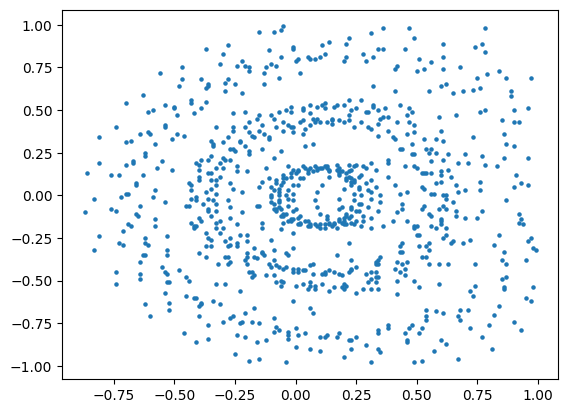
\includegraphics[width=\textwidth]{Chapitre1/Figures/exp1_10_baseH_zoom.png}
                \caption{Graph with zoom of [[-1:1][-1:1]]}
        \end{subfigure}%
        \caption{Resulting of 1000 data statevector}
\end{figure}

\subsubsection{Run 100 full circuit block only}

\begin{figure}[ht!]
        \centering
        \begin{subfigure}[c]{0.5\textwidth}
                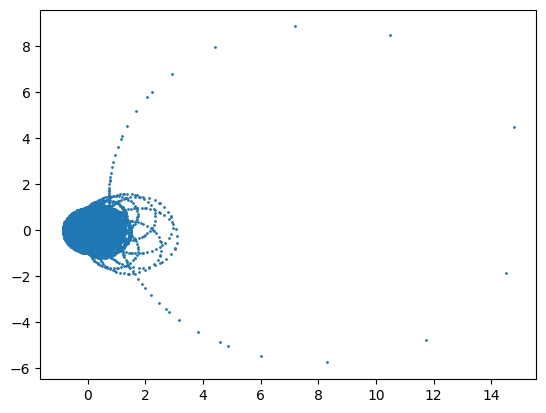
\includegraphics[width=\textwidth]{Chapitre1/Figures/exp1_100_baseH_nonZoom.png}
                \caption{Graph from 10000 data statevector without zoom}
        \end{subfigure}%
        \begin{subfigure}[c]{0.5\textwidth}
                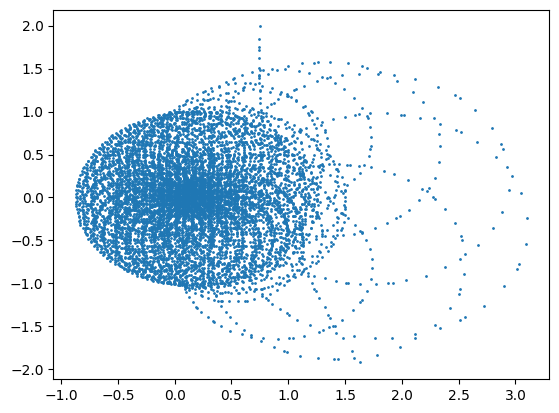
\includegraphics[width=\textwidth]{Chapitre1/Figures/exp1_100_baseH_zoom.png}
                \caption{Graph with zoom of [[-1:2][-1:1]]}
        \end{subfigure}
        \caption{Resulting of 10000 data statevector}
\end{figure}

\subsection{Base H with no-full Z rotation}

\subsubsection{Code}
\begin{lstlisting}
print("Launch!")
qc.h(init_q)
for w in range(max_shots):
    for i in range(shots):
        qc.rx(-pi/(shots-i), init_q)
        qc.rz(pi/(shots/8), init_q)
        z, z_north, z_south = complex_cal(qc, statevector_sim)
        if z != 0:
            if z_north != 0:
                tab_temp[0].append(z)
                tab_temp[1].append(z_north)
            if z_south != 0:
                tab_temp[0].append(z)
                tab_temp[2].append(z_south)
    qc.barrier()
    
    if (w + 1) % 5 == 0:
        print("Full circuit bloch :", w+1, "/", max_shots)

print("Done!")
\end{lstlisting}

\subsubsection{Run 1 full circuit block only}

\subsubsection{Run 10 full circuit block only}
\begin{figure}[ht!]
        \centering
        \begin{subfigure}[c]{0.5\textwidth}
                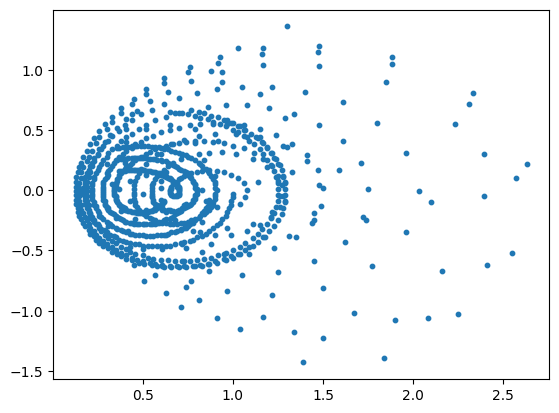
\includegraphics[width=\textwidth]{Chapitre1/Figures/exp1_10_baseH_halfZ_nonZoom.png}
        \end{subfigure}%
        \caption{Resulting of 1000 data statevector}
\end{figure}

\subsubsection{Run 100 full circuit block only}
\begin{figure}[ht!]
        \centering
        \begin{subfigure}[c]{0.5\textwidth}
                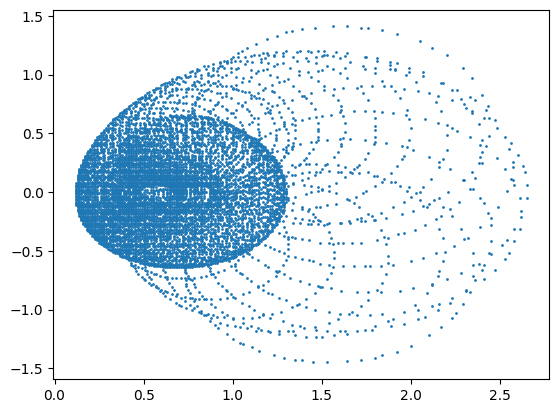
\includegraphics[width=\textwidth]{Chapitre1/Figures/exp1_100_baseH_halfZ_nonZoom.png}
        \end{subfigure}%
        \caption{Resulting of 1000 data statevector}
\end{figure}

\subsection{Base 0}
\subsubsection{Code}
\begin{lstlisting}
print("Launch!")
for w in range(max_shots):
    for i in range(shots):
        qc.rx(-pi/(shots-i), init_q)
        qc.rz(pi/(shots/8), init_q)
        z, z_north, z_south = complex_cal(qc, statevector_sim)
        if z != 0:
            if z_north != 0:
                tab_temp[0].append(z)
                tab_temp[1].append(z_north)
            if z_south != 0:
                tab_temp[0].append(z)
                tab_temp[2].append(z_south)
    qc.barrier()
    
    if (w + 1) % 5 == 0:
        print("Full circuit bloch :", w+1, "/", max_shots)

print("Done!")
\end{lstlisting}

Totototo

\subsubsection{Run 10 full circuit block only}
\begin{figure}[ht!]
        \centering
        \begin{subfigure}[c]{0.5\textwidth}
                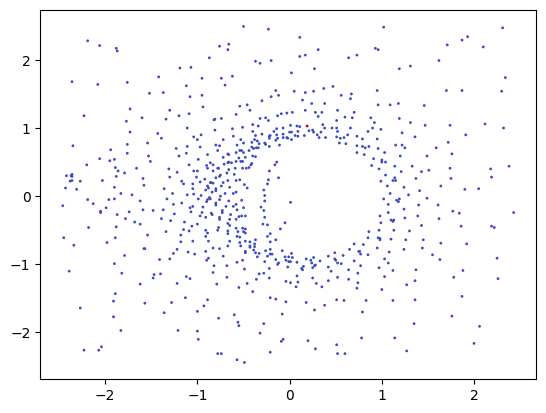
\includegraphics[width=\textwidth]{Chapitre1/Figures/exp1_10_base0_zoom.png}
                \caption{Graph with zoom of [[-2:2][-2:2]]}
        \end{subfigure}%
        \caption{Resulting of 1000 data statevector}
\end{figure}

\subsubsection{Run 100 full circuit block only}
\begin{figure}[ht!]
        \centering
        \begin{subfigure}[c]{0.5\textwidth}
                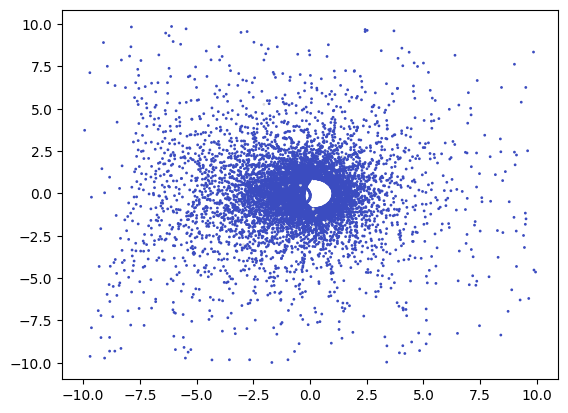
\includegraphics[width=\textwidth]{Chapitre1/Figures/exp1_100_base0_nonZoom.png}
                \caption{Graph from 10000 data statevector without zoom}
        \end{subfigure}%
        \begin{subfigure}[c]{0.5\textwidth}
                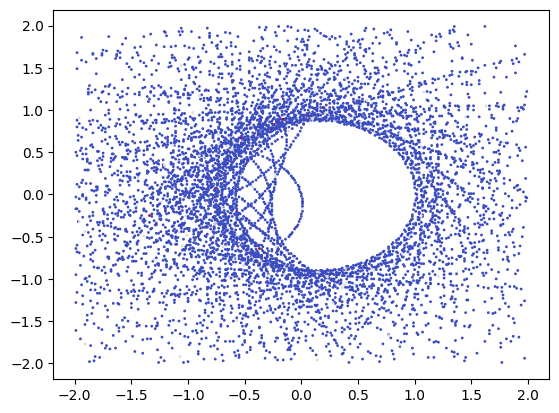
\includegraphics[width=\textwidth]{Chapitre1/Figures/exp1_100_base0_zoom.png}
                \caption{Graph with zoom of [[-2:2][-2:2]]}
        \end{subfigure}
        \caption{Resulting of 10000 data statevector}
\end{figure}





\input{Chapitre2/chapitre2.tex}
\input{Chapitre3/chapitre3.tex}
\input{Chapitre4/chapitre4.tex}
\chapter{Dernier chapitre}
\label{chapter5}

Blablabla.


\chapter*{Conclusion}
\label{chapter:conclusion}
\addcontentsline{toc}{chapter}{Conclusion}

Et voilà !

\bibliographystyle{ieeetr}
\bibliography{biblio}

\end{document}